\documentclass[twocolumns,portrait,a0,final]{a0poster}
%IDIOMAS (PT-BR) E CODIFICAÇÃO DE FONTES
\usepackage[T1]{fontenc}
\usepackage[utf8]{inputenc}
\usepackage[brazilian]{babel}
%OPÇÃO DE FONTES 1 (Padrão)
\usepackage{DejaVuSans}
\renewcommand*\familydefault{\sfdefault}
%OPÇAO DE FONTE 2
\usepackage{lmodern}

%DEFINIÇÃO DO VERDE OFICIAL DOS IFs
\usepackage[svgnames]{xcolor}
\definecolor{verdeOficial}{HTML}{359830}

%CLÁSSICO LOREM IPSUM
\usepackage{lipsum}

%LEGENDAS DAS IMAGENS SEM O AMBIENTE FIGURE
\usepackage{caption}

%IMAGENS
\usepackage{graphicx}

%SEM LINHA DIVISÓRIA PARA \footnote.
\renewcommand{\footnoterule}{}

%URLs
\usepackage{xurl}


%TAMANHO DO PAPEL CONFORME ABNT 15437
%Tam. mín. das margens é 2.5. Padrão para o modelo: como abaixo.
\usepackage[paperwidth=90cm,%
			paperheight=120cm,%
			top=2cm,%
			left=3.5cm,%
			right=3.5cm,%
			bottom=3.5cm,%
			]{geometry}

%TEXTO EM DUAS COLUNAS
\usepackage{multicol}
\setlength{\columnsep}{100pt}         % Distância entre as colunas
\setlength{\columnseprule}{3pt}       % Espessura da linha divisória
\renewcommand{\columnseprulecolor}{\color{verdeOficial}}	% Cor da linhas divisória

%REFERÊNCIAS E CITAÇÕES
\RequirePackage[alf,
				abnt-emphasize=bf,%
				abnt-etal-list=3,%
				abnt-etal-text=emph,%
				abnt-missing-year=sd,%
				abnt-repeated-author-omit=yes,%
				abnt-repeated-title-omit=yes,%
				abnt-thesis-year=final,%
				abnt-doi=link,%
				]{abntex2cite}
%ALTERAR O TAMANHO DA FONTE APÓS BIBLIOG. COMPILADA
\let\oldthebibliography\thebibliography
\let\endoldthebibliography\endthebibliography
\renewenvironment{thebibliography}[1]
{\normalsize\oldthebibliography{#1}}
{\endoldthebibliography}

%CAIXAS DE TEXTO PADRÃO (SEÇÕES DO PÔSTER)
\usepackage{tcolorbox}
\tcbuselibrary{many}
\tcbset{colback=green!5!white,%
		colframe=green!60!black,%
		fonttitle=\bfseries\large,%
		toprule=5mm,%
		rightrule=3mm,%
}

%CAIXA DE AGRADECIENTOS
\usepackage{awesomebox}
\newcommand{\agradecimentos}[1]{%
	\awesomebox[verdeOficial][][\textbf{\color{verdeOficial}{Agradecimentos}}]%
	{2pt}{\faThumbsUp}{verdeOficial}{#1}%
}

%DEFINIÇÃO DO RODAPÉ (LINHA)
%(RE)Fazer o cabeçalho usando apenas esse pacote, sem o minipage.
\usepackage{fancyhdr}
\renewcommand{\headrulewidth}{0.0pt}
\renewcommand{\footrulewidth}{1pt}
\renewcommand{\footrule}{%
	{\color{verdeOficial}\hrule width\headwidth height\footrulewidth}%
	\vskip\footruleskip%
}
\fancyfoot{}


%INFORMAÇÃO PÔSTER
\author{Autor}
\title{Título}
\date{; data@email.com}

\begin{document}
\pagestyle{fancy}
{\color{verdeOficial}\hrule height 5pt}
\vspace{0.5cm}
\begin{minipage}{10cm}
\begin{center}
	
\includegraphics[width=7cm]{./img/logo-ifpe.png}
\end{center}
\end{minipage}
\begin{minipage}{63cm}
	\begin{center}% PREENCHER A IDENTIFICAÇÃO DO PÔSTER+AUTOR+E-MAIL ABAIXO
		{\Huge\bfseries Título Gigante do Poster}\\%
		{\LARGE Autorão Exemplar 1\footnote{data1@email.com}; Autorão Exemplar 2\footnote{data2@email.com};Autorão Exemplar 3\footnote{data3@email.com}}\\%
	\end{center}
\end{minipage}
\begin{minipage}{10cm}
	\begin{flushleft}
		
\includegraphics[width=8cm]{./img/logo-do-evento.png}
	\end{flushleft}
\end{minipage}
{\color{verdeOficial}\hrule height 5pt}
\ \\
{\color{verdeOficial}\hrule height 5pt}
\ \\

%Introdução, Metodologia, Resultados e Discussão, Conclusão e Referências 
%INÍCIO DO TEXTO EM DUAS COLUNAS. SUBSTITUIR O COMANDO \lispum[1] PELO TEXTO.
\begin{multicols}{2}
\begin{tcolorbox}[title=\section{INTRODUÇÃO}]
	\lipsum[1]
\end{tcolorbox}
\vspace{1cm}

\begin{tcolorbox}[title=\section{METODOLOGIA}]
	\lipsum[1]
\end{tcolorbox}
\vspace{1cm}

\begin{tcolorbox}[title=\section{RESULTADOS E DISCUSSÃO}]
	\lipsum[1]
\end{tcolorbox}
\vspace{1cm}

%POSICIONAMENTO DE IMAGENS
%Adequar às necessidades
% 1. DUAS IMAGENS LADO A LADO (larguras iguais)
\begin{minipage}{0.48\linewidth}
	\centering
	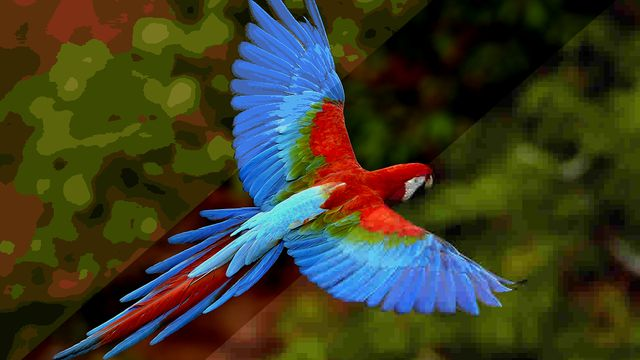
\includegraphics[width=\linewidth]{./img/imagem-exemplo.jpeg}
	\captionof{figure}{Legenda da imagem 1}
\end{minipage}
\hfill
\begin{minipage}{0.48\linewidth}
	\centering
	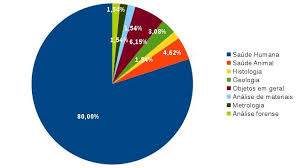
\includegraphics[width=\linewidth]{./img/grafico-pizza.jpeg}
	\captionof{figure}{Legenda da imagem 2}
\end{minipage}

\vspace{0.5cm}

% 2. IMAGEM ABAIXO DA OUTRA (largura total)
\begin{center}
	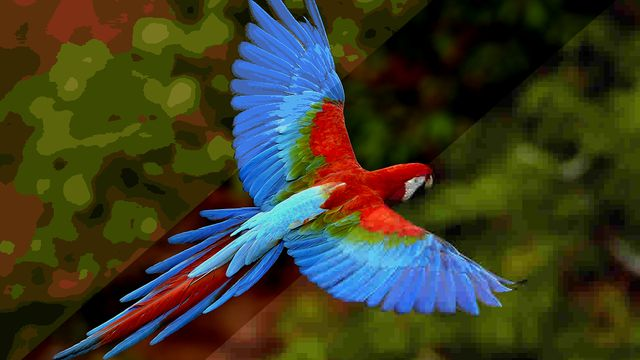
\includegraphics[width=\linewidth]{./img/imagem-exemplo.jpeg}
	\captionof{figure}{Legenda da imagem 1}
	
	\vspace{0.5cm}
	
	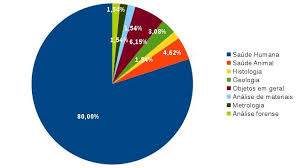
\includegraphics[width=\linewidth]{./img/grafico-pizza.jpeg}
	\captionof{figure}{Legenda da imagem 2}
\end{center}

% 3. IMAGEM ABAIXO DA OUTRA (largura customizada)
\begin{center}
	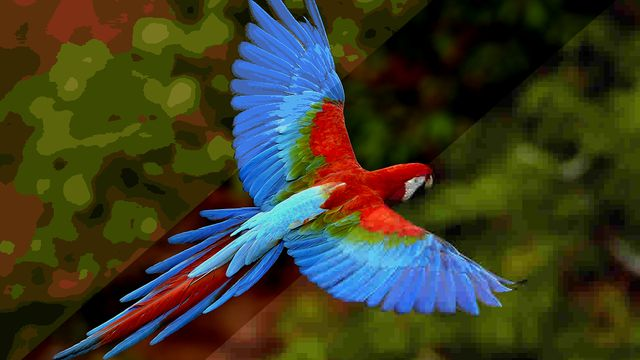
\includegraphics[width=0.8\linewidth]{./img/imagem-exemplo.jpeg}
	\captionof{figure}{Legenda da imagem 1}
	
	\vspace{0.5cm}
	
	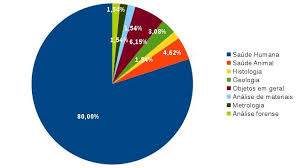
\includegraphics[width=0.8\linewidth]{./img/grafico-pizza.jpeg}
	\captionof{figure}{Legenda da imagem 2}
\end{center}
%POSICIONAMENTO DE IMAGENS

\begin{tcolorbox}[title=\section{CONCLUSÃO}]
	\cite{loki2019} e depois \cite{thor2020}
\end{tcolorbox}
\vspace{1cm}

%PRODUZIR AS REFERÊNCIAS
\begin{tcolorbox}
	\renewcommand{\bibname}{Referências}
	\bibliographystyle{abntex2-alf}
	\bibliography{referencias-poster}
\end{tcolorbox}
\vspace{1cm}

\agradecimentos{Agradeço a ... \lipsum[2]}

\end{multicols}
\end{document}
